\documentclass{article}
\usepackage[utf8]{inputenc}
\usepackage{listings}
\usepackage{graphicx}
\usepackage{color}
\usepackage[usenames,dvipsnames]{xcolor}
\usepackage{placeins}
\usepackage{epstopdf}
\DeclareGraphicsExtensions{.eps}
\usepackage{fullpage}

\title{Bayesian Analysis of Survival Probability in \\ \textit{A Song of Ice and Fire}}
\author{Erin Pierce and Ben Kahle}
\date{December 2014}

\begin{document}

\maketitle

\section{Introduction}


The Song of Ice and Fire Series has a reputation for being quite deadly.  No character, good or bad, major or minor is safe from Martin's pen.  The reputation is not unwarranted; of the 916 named characters that populate Martin's world, a third have died, alongside countless nameless ones. For our Bayesian case study, we wanted to take a closer look at the patterns of death in the novels and create a Bayesian model that would allow us to predict the probability that characters will survive the next two novels. We first had to create a data set of all 916 characters that appeared in the books so far.  For every character, we know what chapter and book they first appeared, if they are male or female, if they are part of the nobility or not, what major house they are loyal to, and, if applicable, the chapter and book of their death. This data set was created from http://awoiaf.westeros.org/ by a combination of scraping and manual collection. We then used to data to make predictions about which characters will survive the next couple books.

\section{An Example of The Process}

In our data set, we optimistically kept Jon Snow as alive. By looking at the survival patterns of the sworn brothers of the Night's Watch demonstrate how reasonable this outcome is.  From the data set, we can study the 116 men who have allegiance to the Night's Watch.  For each one that is dead as of the end of a Dance with Dragons we account for the chapter they were introduced and the chapter they died in order to calculate the character's "age". All introductions are assumed to have happened at the beginning of the chapter and deaths are assumed to have happened at the end of the chapter.  Then, based on the number of chapters in the book, we calculate at what percentage through the book the introduction/death occurred.  From the difference of these two numbers we get a lifetime for that character.  In doing this we are making some strange assumptions about each book being an equal amount of time or plot or pages, and each chapter being the same length, however this still provides a reasonable age resolution given the data available. An example of these calculations can be seen through the character of Jeor Mormont.  Mormont is first introduced when Jon Snow is assigned to be his steward, in ch. 48 of \textit{A Game of Thrones}.  He is killed in the mutiny at Craster's keep, which occurs ch. 33 of \textit{A Storm of Swords}. There are 72 chapters in \textit{A Game of Thrones} and 81 in \textit{A Storm of Swords} so his lifetime is calculated as:
$$
\bigg( 2+ \frac{34}{81} \bigg) - \bigg(0+\frac{48}{72}\bigg) = 1.75
$$

For the brothers that are still alive, the ages are calculated at the end of \textit{A Dance with Dragons} in much the same way.  These lifetimes and ages are in units of books, and have nothing do with the characters physical ages.

We then use these lifetimes and ages to do a Kaplan-Meier estimation. This provides us with a survival curve and a hazard function for the Night's Watch. The survival curve, evaluated at an individual character's age, is the probability that a character will have a lifetime greater than that age, and the hazard function, evaluated at a individual character's age, is the probability that a character had a lifetime that long. Kaplan-Meier is used because it can model a population that includes both dead people (who's lifetime is know) and living people (who's current age is known).


\begin{figure}[ht!]
\centering
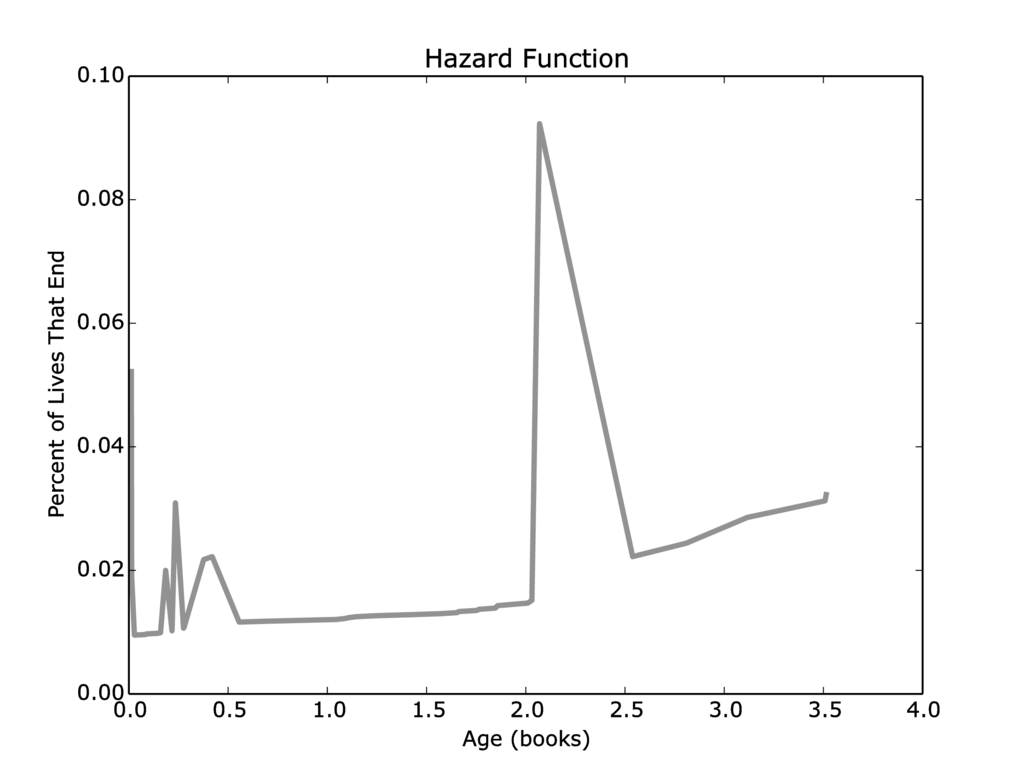
\includegraphics[width=4in]{NWHaz.png}
\caption{Many men of the Night's Watch die in the same book they are introduced.  The spike around two books are due to the many new brothers introduced when Jon took the black, and the many brothers killed at the fist of the first men and the ensuing chaos in the first half of \textit{A Storm of Swords}.}
\label{fig:nwhaz}
\end{figure}



\begin{figure}[ht!]
\centering
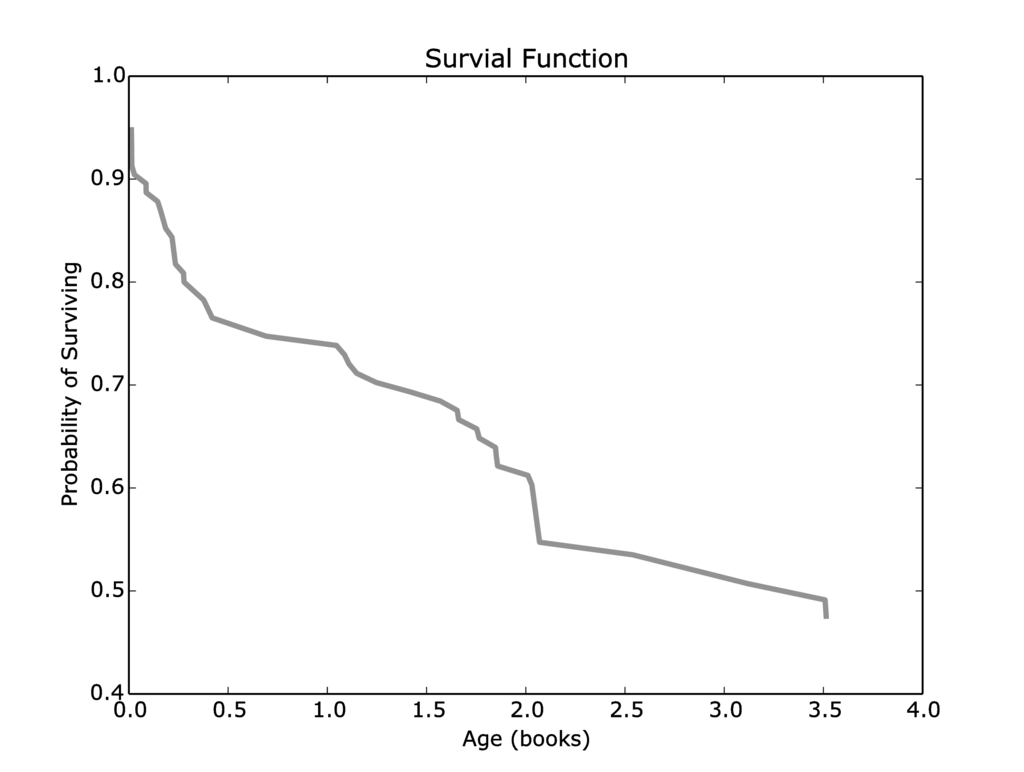
\includegraphics[width=4in]{NWSurv.png}
\caption{The smoother survival curve shows that the chance of survival decrease dramatically initially, but if a character has survived for more than about 2 books, their chance of survival begins to levels out.}
\label{fig:nwsurv}
\end{figure}

The curves do not extend all the way to 5 books because there are no dead characters who lived that long. The oldest dead brother was 3.51 books old.  It was Dareon, a bard of the Night's Watch known for his singing voice who was in the same novice class as Jon, and was introduced early in \textit{Game of Thrones}.  He then deserted the watch and worked as singer in Braavos, where he was eventually killed by Arya towards the end of \textit{A Feast for Crows}.

The survival and hazard functions are a good way to represent the available data, but addtional modeling enable predictions about characters living more than a few books.

A Weibull distribution provides a way to model the Kaplan-Meier estimation.  The Weibull distribution depends on two parameters, k and lambda, which control its shape.  The PDF of the Weibull distribution is the hazard function, and the inverse of the CDF of the Weibull distribution is the survival curve.  As seen in the comparison of Figures \ref{fig:nwhaz} and \ref{fig:nwsurv}, the survival curve tends to be smoother and lends itself to mathematical approximation better than the hazard function. 

For both parameters k and lambda we began with a uniform prior.  Iterating through each alive character, we checked how well that value of k or lambda predicted the fact that the character was still alive.  For each dead character, we checked how well the parameters predicted the time of their death.  For the Night's Watch, this lead to the posterior distribution in Figure \ref{fig:NW_post}. The main code used to update these distributes is the following:
\lstset{language=Python,
        numbers=left,
        frame=none,
        morecomment=[l]{//},
        backgroundcolor=\color{white},   % choose the background color t
        basicstyle=\footnotesize,        % size of fonts used for the code
        breaklines=true,                 % automatic line breaking only at whitespace
        captionpos=b,                    % sets the caption-position to bottom
        commentstyle=\color{mygreen},    % comment style
        escapeinside={\%*}{*)},          % if you want to add LaTeX within your code
        keywordstyle=\color{blue},       % keyword style
        stringstyle=\color{ForestGreen},     % string literal style
        basicstyle=\footnotesize\ttfamily, % fixed-width font
        showstringspaces=false
}
\begin{lstlisting}
class GOT(thinkbayes2.Suite, thinkbayes2.Joint):

	def Likelihood(self, data, hypo):
		"""Determines how well a given k and lam predict the life/death of a character """
		age, alive = data
		k, lam = hypo
		if alive:
			prob = 1-exponweib.cdf(age, k, lam)
		else:
			prob = exponweib.pdf(age, k, lam)
		return prob

def Update(k, lam, age, alive):
	"""Preforms the Baysian Update and returns the PMFS of k and lam"""
	joint = thinkbayes2.MakeJoint(k, lam)
	suite = GOT(joint)
	suite.Update((age, alive))
	k, lam = suite.Marginal(0, label=k.label), suite.Marginal(1, label=lam.label)
	return k, lam

def MakeDistr(introductions, lifetimes,k,lam):
	"""Iterates through all the characters for a given k and lambda.  It then updates the k and lambda distributions"""
	k.label = 'K'
	lam.label = 'Lam'
	print("Updating deaths")
	for age in lifetimes:
		k, lam = Update(k, lam, age, False)
	print('Updating alives')
	for age in introductions:
		k, lam = Update(k, lam, age, True)
	return k,lam
\end{lstlisting}

To translate this back to a survival curve, we took the mean of k and lambda, as well as the 90 percent credible interval for each parameter.  The mean is fairly straightforward, but taking the credible interval for both distributions leaves us with four possible permutations of upper and lower bounds.  By visual inspection, we decided that the lower bound of the survival curve used the higher value of lambda and the lower value of k while The upper bound used the lower value of lambda and the higher value of k.  We can then plot the original data, the credible interval, and the single curve generated from the means as seen in many of the figures below.

\begin{figure}[ht!]
\centering
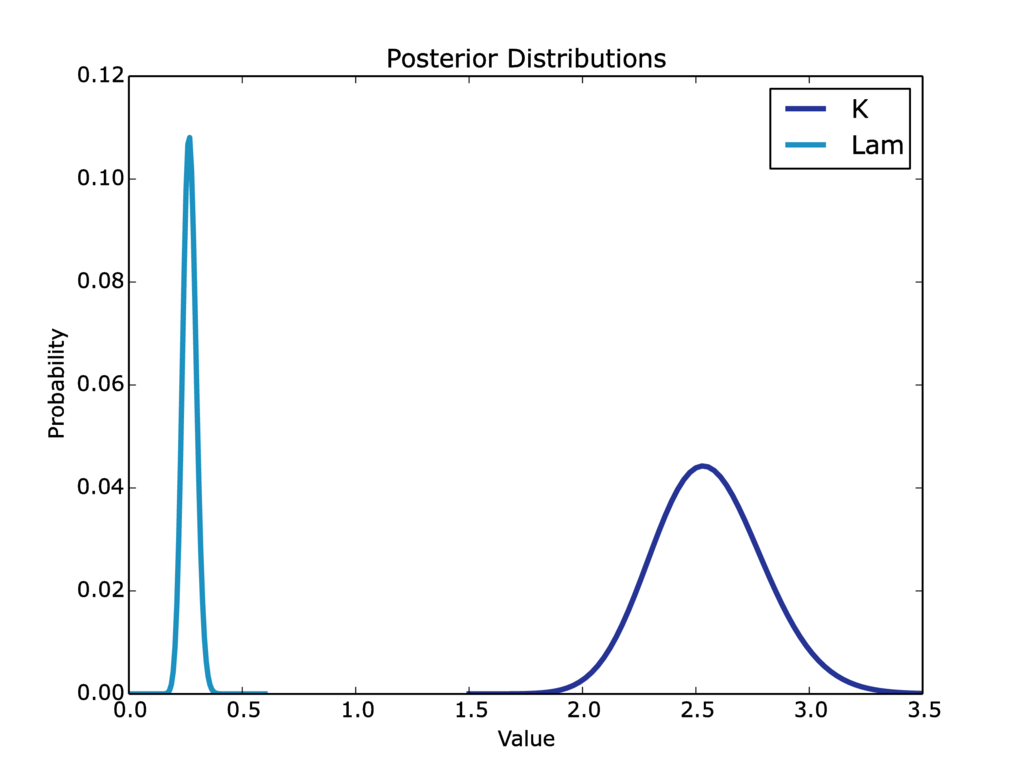
\includegraphics[width=4.5in]{NWK_lam.png}
\caption{The distribution for lambda is quite tight, around 0.27, but the distribution for k is broader.}
\label{fig:NW_post}
\end{figure}

 \begin{figure}[ht!]
\centering
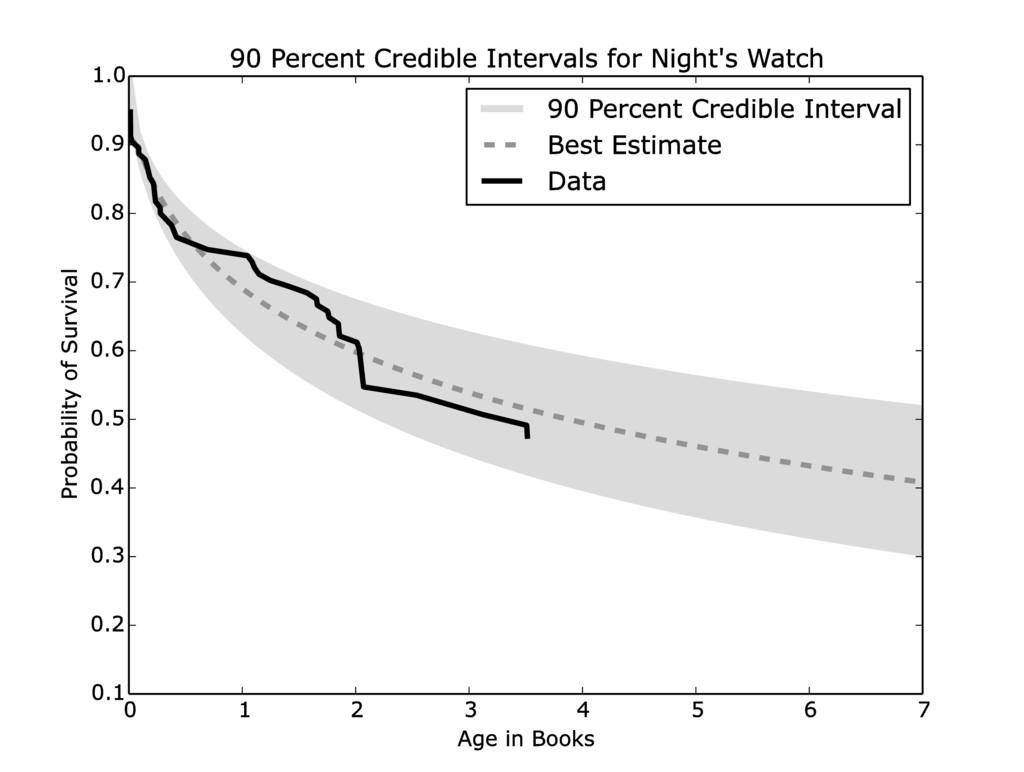
\includegraphics[width=5in]{NWExp.png}
\caption{The credible interval closely encases the data, and the mean-value curve appears to be a reasonable approximation.}
\label{fig:nwcred}
\end{figure}

\newpage

Using this analysis, we can can begin to make a prediction for an individual character like Jon Snow.  At the end of \textit{A Dance with Dragons}, the credible interval for the Night's Watch survival (Figure \ref{fig:nwcred}) stretches from 36 percent to 56 percent.  The odds are not exactly rosy that Jon snow is still alive.  Even if Jon is still alive at the end of book 5, the odds that he will survive the next two books drop to between 30 percent and 51 percent. However, it is also worth considering that Jon is not an average member of the Night's Watch.  He had a noble upbringing and is well trained at arms. We repeated the same analysis with only members of the Night's Watch considered noble due to their family, rank, or upbringing.

There have only been 11 nobles in the Night's Watch, so the credible interval as seen in Figure \ref{fig:nwnobelcred} is understandably much wider, however, the best approximation of the survival curve suggests that a noble background does not increase the survival rate for brothers of the Night's Watch.

 \begin{figure}[ht!]
\centering
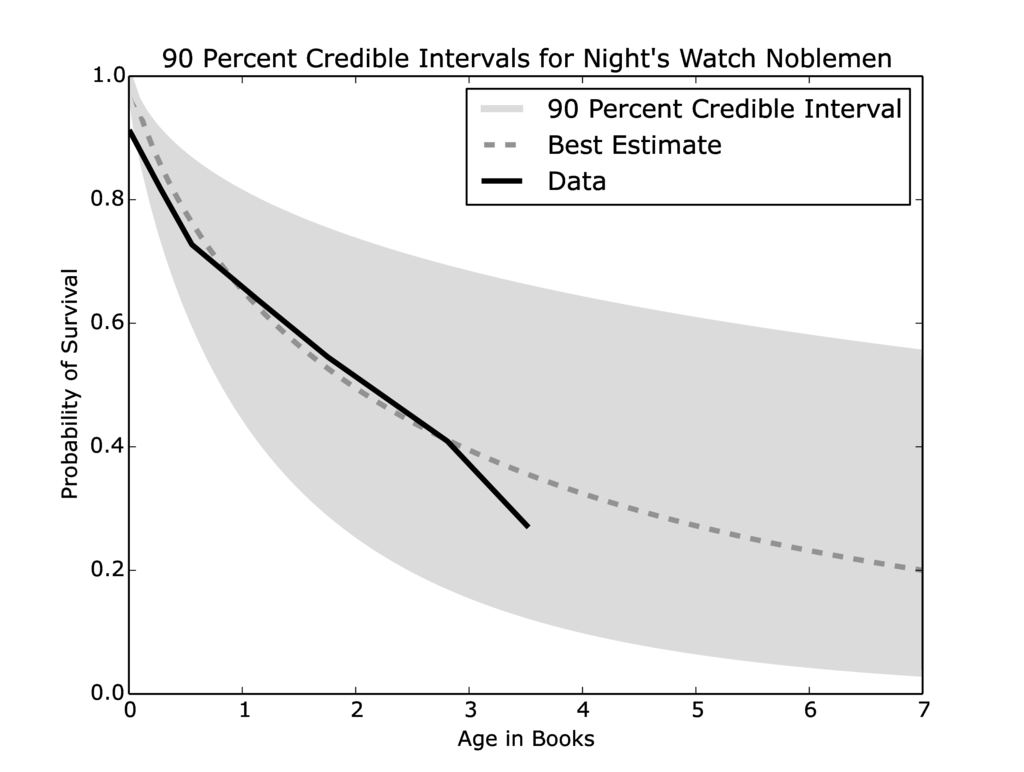
\includegraphics[width=5in]{NWNExp.png}
\caption{When only nobel members of the Night's Watch are included, the credible interval widens significantly and the lower bound gets quite close to zero.}
\label{fig:nwnobelcred}
\end{figure}

\section{Our Results}
\subsection{Houses}

The 90 percent credible intervals for all of the major houses.  This includes the 9 major houses, the Night's Watch, the Wildlings, and a "None" category which includes non-allied characters.

\begin{figure}[ht!]
\centering
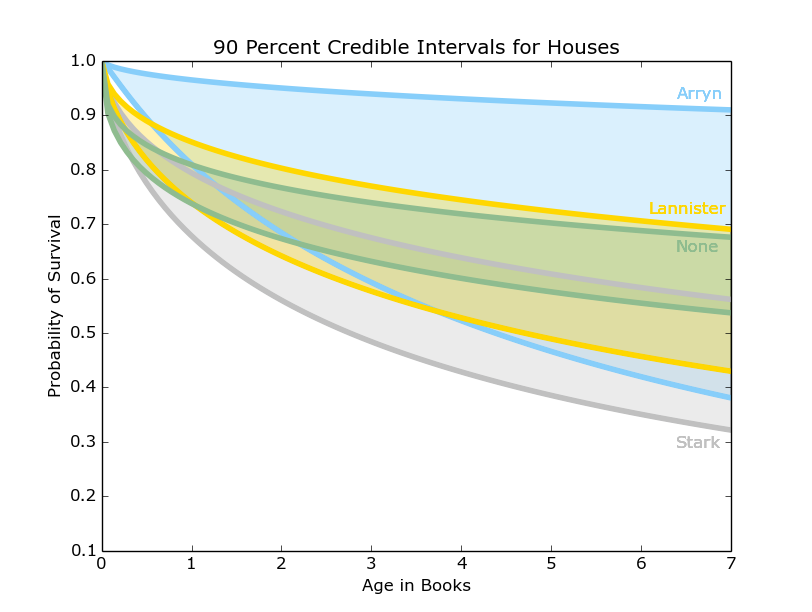
\includegraphics[width=4.8in]{House1.png}
\caption{90 percent credible interval for Arryn (Blue), Lannister (Gold), None (Green), and Stark (Grey)}
\label{fig:house1}
\end{figure}

\begin{figure}[ht!]
\centering
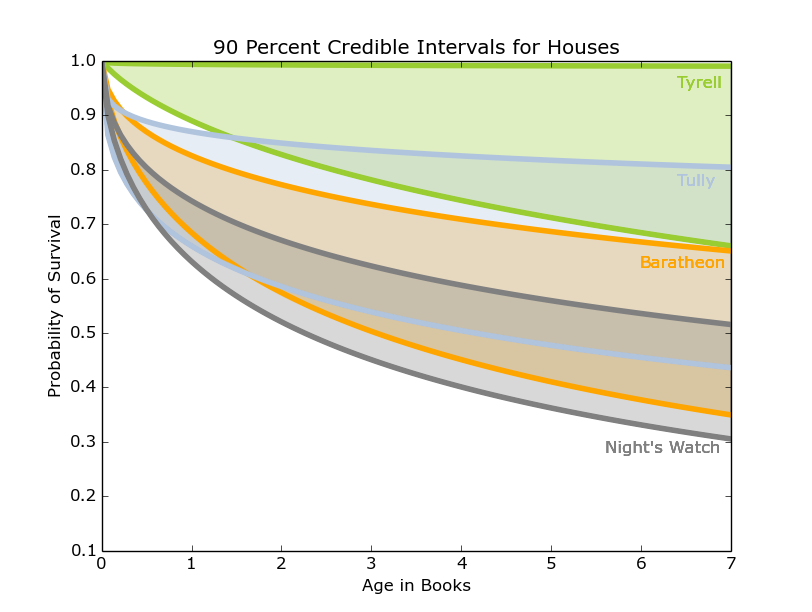
\includegraphics[width=4.8in]{Houses2.png}
\caption{90 percent credible interval for Tyrell(Green), Tully(Blue), Baratheon(Orange), and Night's Watch (Grey)}
\label{fig:house2}
\end{figure}

\begin{figure}[ht!]
\centering
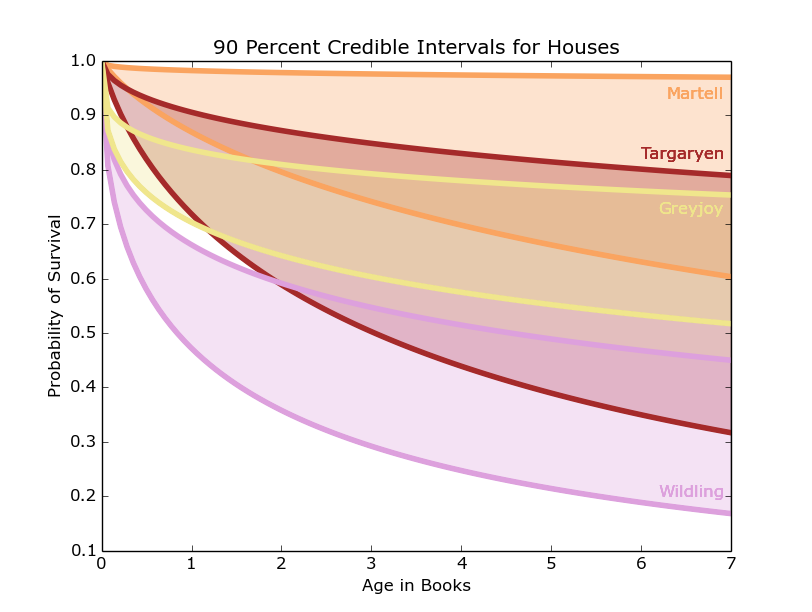
\includegraphics[width=4.8in]{Houses3.png}
\caption{90 percent credible interval for Martell(Orange), Targaryen (Maroon), Greyjoy (Yellow), and Wildling (Purple)}
\label{fig:house3}
\end{figure}

\newpage

These intervals, shown in Figures \ref{fig:house1}, \ref{fig:house2}, and \ref{fig:house3}, demonstrate a much higher survival probability for the houses Arryn, Tyrell, and Martell. Supporting these results, these houses have stayed out of most of the major conflicts in the books, however this also means there is less information on them.  We have 5 or less examples of dead members for those houses, so the survival curves don't have very many points.  This uncertainty is reflected in the wide credible intervals.

In contrast, our friends in the north, the Starks, Night's Watch, and Wildlings have the lowest projected survival rates and smaller credible intervals given their warring positions in the story and the many important characters included amongst their ranks.  This analysis considers entire houses, but there are also additional ways to sort the characters.

\subsection{Gender}
While A Song of Ice and Fire has been lauded for portraying women as complex characters who take an a variety of roles, there are still many more male characters (769) than female ones (157). Despite a wider credible interval, the women tend to fare better than their male counterparts, out-surviving them by a fair degree as seen in Figure \ref{fig:gender}.
\newpage
\begin{figure}[ht!]
\centering
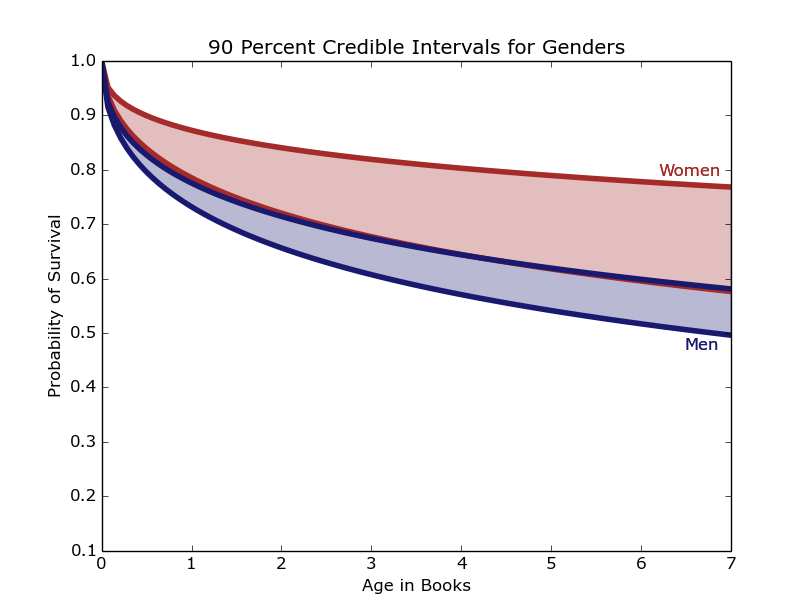
\includegraphics[width=4in]{Gender.png}
\caption{The women of Westeros appear to have a better chance of surviving then the men.}
\label{fig:gender}
\end{figure}

\subsection{Class}
The ratio between noble characters(429) and smallfolk characters (487) is much more even than gender and provides an interesting comparison for analysis. Figure \ref{fig:class} suggests that while more smallfolk tend to die quickly after being introduced, those that survive their introductions tend to live for a longer period of time and may in fact outpace the nobles.

\begin{figure}[ht!]
\centering
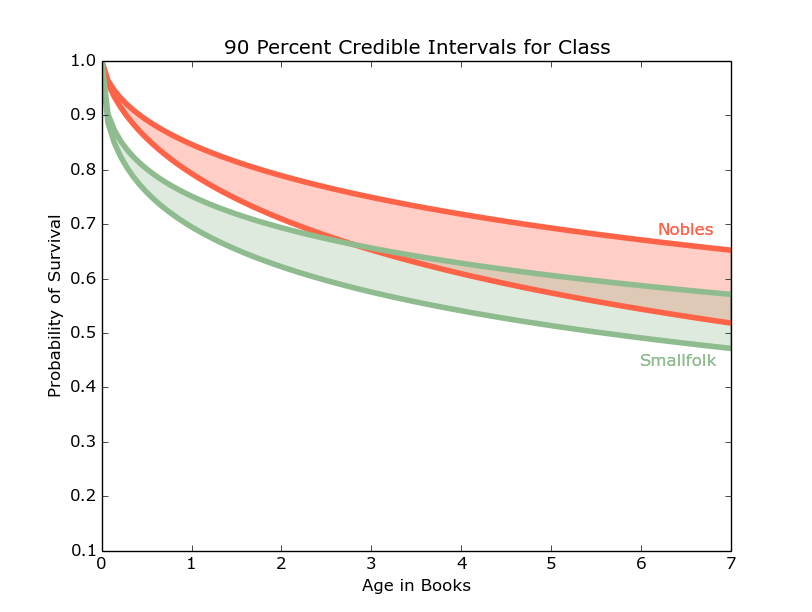
\includegraphics[width=4in]{Class.png}
\caption{The nobility might have a slight advantage when introduced, but their survival probability continues to fall while the smallfolk's levels much more quickly}
\label{fig:class}
\end{figure}

\subsection{Specific Characters}

The same analysis can be extended to combine traits, sorting by gender, house, and class to provide a rough model for individual characters.
One of the most popular characters in the books is Arya and many readers are curious about her fate in the books to come. The category of noblewomen loyal to the Starks also includes other noteworthy characters like Sansa and Brienne of Tarth (though she was introduced later). Other intriguing characters to investigate are the Lannister noblewomen Cersei and poor Myrcella.  As it turns out, not a lot noble women die.  In order to get more precise credible intervals for the specific female characters we included the data of both noble and smallfolk women. 

\begin{figure}[ht!]
\centering
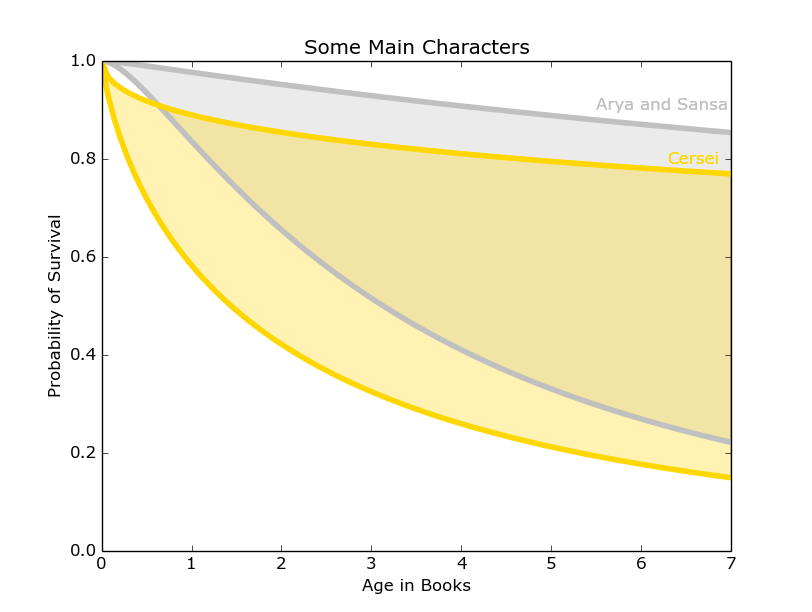
\includegraphics[width=6in]{Fem1.png}
\caption{While both groups have very wide ranges of survival probabilities, the Lanister noblewomen may be a bit more likely to die than the Starks.}
\label{fig:specwomen}
\end{figure}

The data presented in Figure \ref{fig:specwomen} is fairly inconclusive for both groups, however it does looks like Arya has a slightly better chance of survival than Cersei. Two minor characters we were curious about were Val, the wildling princess, and the mysterious Quaithe. 
\newpage

\begin{figure}[ht!]
\centering
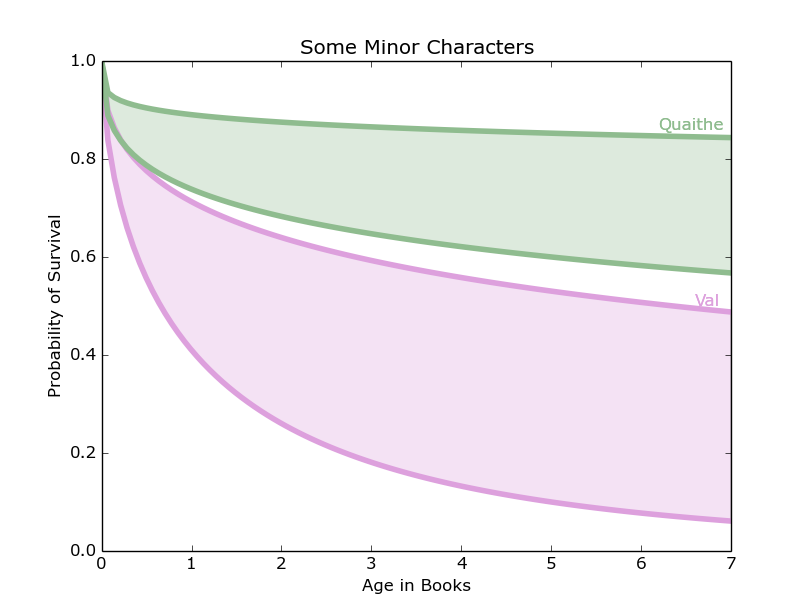
\includegraphics[width=6in]{Fem2.png}
\caption{Representing the survival curves of more minor characters, Quaithe and Val have dramatically different odds of surviving the series.}
\label{fig:minorwomen}
\end{figure}
They both had more data than the Starks and Lannisters, but they have the complication that they were not introduced at the beginning of \textit{A Game of Thrones}. Val is introduced at 2.1 books, and so Val's chances of surviving the whole series are between 10 percent and 53 percent, which are not the most inspiring of chances.  Quaithe is introduced at 1.2 books, and her chances are between 58 percent and 85 percent, which is significantly better than Val's. These curves, shown in Figure \ref{fig:minorwomen}, are some of the most distinct amongst the data set.
\newpage

For most of the male characters (with the exception of Mance), there was enough data to narrow to house, gender and class.

\begin{figure}[ht!]
\centering
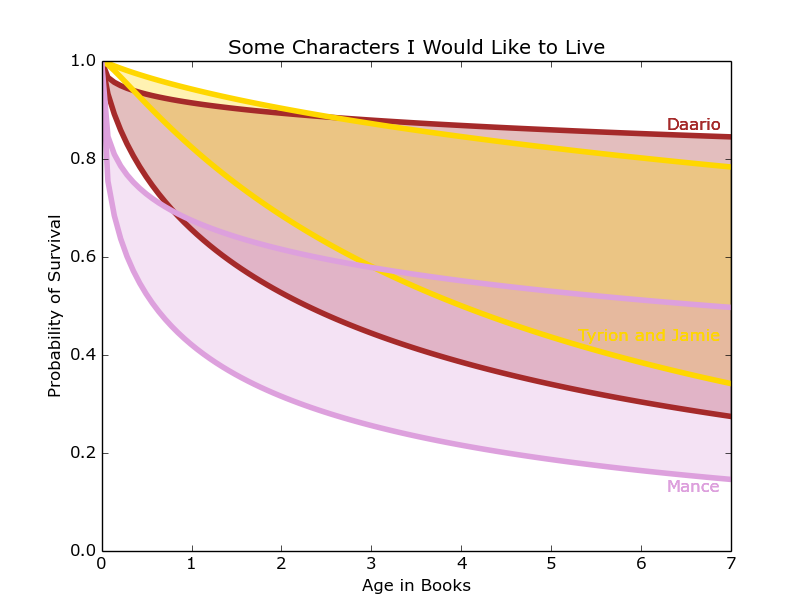
\includegraphics[width=6in]{Male1.png}
\caption{The survival curves of different classes and alliances of men shown through various characters.}
\label{fig:male1}
\end{figure}

Figure \ref{fig:male1} shows the Lannister brothers with middling survival chances ranging from 35 percent to 79 percent.  The data for Daario is less conclusive, but seems hopeful, especially considering he was introduced at 2.5 books. Mance seems to have to worst chance of surviving till the end.  He was introduced at 2.2 books, giving him a chance of survival between 19 percent and 56 percent.

\newpage

\begin{figure}[ht!]
\centering
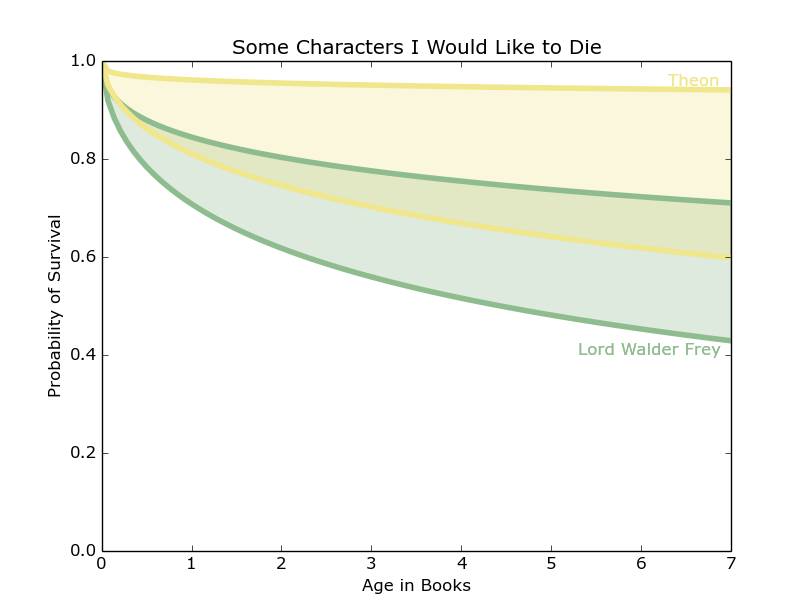
\includegraphics[width=6in]{Male2.png}
\caption{The survival curves of different classes and alliances of men shown through various characters}
\label{fig:male2}
\end{figure}
Some characters who many wouldn't mind seeing kick the bucket include Lord Walder Frey and Theon Greyjoy. However, Figure \ref{fig:male2} suggests that neither are very likely meet untimely (or in Walder Frey's case, very timely) deaths.  Theon seems likely to survive to the bitter end.  Walder Frey was introduced at 0.4 books, putting his chances at 44 percent to 72 percent. As it is now, Hoster Tully may be the only character that has died of old age, so perhaps Frey will hold out until the end.

\section{Notes on the Data Set}
Most characters were fairly easy to sort, but there are always edge cases.
\begin{enumerate}
\item Gender - This was the most straight forward.  There are not really any gender-ambigous characters.
\item Nobility - Members of major and minor Westeros houses were counted as noble, but hedge knights were not.  For characters from Essos, I used by best judgement based on money and power, and it was usually an easy call.  For the wildlings, I named military leaders as noble, though that was often a blurry line. For members of the Night's Watch, I looked at their status before joining in the same way I looked at other Westeros characters.  For bastards, we decided on a case by case basis.  Bastards who were raised in a noble family and who received the education and training of nobles were counted as noble.  Thus Jon Snow was counted as noble, but someone like Gendry was not.
\item Death - Characters that have come back alive-ish (like Beric Dondarrion) were judged dead at the time of their first death.  Wights are not considered alive, but others are. For major characters whose deaths are uncertain, we argued and made a case by case decision.
\item Houses - This was the trickiest one because some people have allegiances to multiple houses or have switched loyalties. We decided on a case by case basis.  The people with no allegiance were of three main groups:
    \begin{itemize}
        \item People in Essos who are not loyal to the Targaryens.
        \item People in the Riverlands, either smallfolk who's loyalty is not known, or groups like the Brotherhood Without Banners or the Brave Companions with ambiguous loyalty.
        \item Nobility that are mostly looking out for their own interests, like the Freys, Ramsay Bolton, or Petyr Baelish. 
    \end{itemize}
\end{enumerate}
\section{Conclusion}
Of course who lives and who dies in the next two books has a lot more to do with plot and storyline than with statistics.  Nonetheless, using our data we were able we were able to see distinct patterns of life and death among various groups of characters.  For some characters, especially males, we were able to get fairly specific predictions of how they will fare in the next novels, though the verdict is still out on characters for less discussed houses and many female characters.

The code used in the case study can be found at: \\
http://github.com/benkahle/bayesianGameofThrones

\end{document}
